\clearpage
\graphicspath{{./lib/message_handler/figures/}}
\acresetall

\section{Message Handler}
\label{lib:messagehandler}

\begin{refsection}
\begin{tcolorbox}	
	\begin{tabular}{p{2.75cm} p{0.2cm} p{10.5cm}} 	
    	\textbf{Header Files}    &:& message\_handler.h \\
		\textbf{Source File}     &:& message\_handler.cpp \\
	\end{tabular}
\end{tcolorbox}

\subsection{Introduction}
A Message Handler is a Block/Program responsible for receiving and 
transmitting message objects to other Blocks/Programs.
The generic implementation of this Block is depicted in 
\autoref{fig:Handler_Block}. 
\\
\begin{figure}[!b]
	\centering
	\includegraphics[width=1\linewidth]{message_Handler_generic.png}
	\caption{Message Handler Block}
	\label{fig:Handler_Block}
\end{figure}
\\
A simple description of it's job is to collect messages from the input 
signals and place them in the Internal Buffers, according to their 
destination. Then, ordered by the priority and order of insertion, remove
those messages from the buffers and place them in the output signals.
\\
\textbf{Note:} As present in the \textit{Netxpto} file, a Block is just a
representation of a components/program. This Components are interconnected 
using a Signal, which is an object that allows them to share a memory space
(Circular Buffer) for exchanging data.

\subsection{Input Signals}
There are no mandatory Input Signals for the Message Handler, as it can 
function with at least one. This Signals are used to get the messages, that are with
then saved in the Internal Buffers

\subsection{Output Signals}
Like the Input Signals, there are also no mandatory Output Signals, allowing it 
to function with at least one. The Output Signals are used to send the messages 
according to their location. The Message Handler will create one Internal 
Buffer for each Output Signal, allowing it to continue to function and to not 
lose messages during high processing times.

\subsection{Class t\_handler\_message}
\label{lib:t_handler_message}

This class resides in the \textbf{NetXpto} module and was created to replace the previous 
\textit{t\_message} class. This new class implements more macros, abilities (with operator 
functions) and information about the message encoded in the header. 
\\
The new Message Format is defined in \autoref{table:Message_format_Handler}. 
There are also macros indicating the sizes, in bytes, present in the table.
\\
\begin{table}[H]
	\centering
	\begin{tabular}{|m{0.1\textwidth}|m{0.2\textwidth}|m{0.1\textwidth}|m{0.5\textwidth}|}
		\cline{1-4}
		\textbf{Group} & \textbf{Field Name} & \textbf{Bytes} & \textbf{Observation}\\ \cline{1-4}
		Header & dstBlock & 32 & Name of the Destination Block. Parameter used to route the Message \\ \cline{1-4}
		Header & srcBlock & 32 & Name of the Block that generated the Message \\ \cline{1-4}
		Header & priority & 1 & Defined between [0-5], from Low to High Priority, respectively\\ \cline{1-4}
		Header & ID & 4 & Sequential Id assigned by the Source Block \\ \cline{1-4}
		Header & messageType & 35 & Type of the message, defined by the Source Block \\ \cline{1-4}
		Header & srcPort & 1 & Assigned by the Message Handler, before placing the message in it's buffer \\ \cline{1-4}
		Header & dataLength & 6 & Length of the Data field in the message \\ \cline{1-4}
		Data & Data & 5000 & Payload or data to be transmitted \\ \cline{1-4}
	\end{tabular}
	\caption{Message Format defined in the class t\_handler\_message}
	\label{table:Message_format_Handler}
\end{table}

\subsubsection{Operator functions}
Operator functions are default functions used to make operations or actions
between one or two object of the same class. Since the messages will be placed
and ordered based on attributes, in the Message Handler and Signal buffers, 
the following functions were created:
\begin{itemize}
	\item \textit{operator<}: This function compares two messages and returns 
		\textbf{true} if the current message is less than the other
	\item \textit{operator==}: This function compares two messages and returns 
		\textbf{true} if they are equal
	\item \textit{operator=}: This function copies the content of the second
		message into the first one and returns the reference to the first one
	\item \textit{operator<<}: This function is used to write the contents of 
		a message, into a out stream object
	\item \textit{operator[]}: This function provides array-like access to this
		class
\end{itemize}

\subsubsection{Interaction with signals}
The Signals and Base Signals classes are located in the \textit{Netxpto} file 
and use Enum classes already defined there, we needed to add this new class
to the possible types of the Signals buffers. This can be seen as a 
circular dependency, where this component depends on the \textit{Netxpto} 
component and it depends on this one. However that is not the case, the 
changes in the \textit{Netxpto} were only to the \textit{signal\_value\_type}
and \textit{signal\_type} classes, as well as to the \textit{Signal::setType}
function. This changes make no impact on previous code and allow the 
declaration of the \textbf{HandlerMessage} signal in this component, to be used
as a Signal.

Due to the architecture and functions used by the Signals and BaseSignals to 
insert and remove messages from the Signals, new functions \textbf{bufferPut} 
and \textbf{bufferGet} for the \nameref{lib:t_handler_message} needed to be created.
So that demanded for this new classes to be located in the \textit{Netxpto} file.

\subsection{Class PriorityBuffer}
\label{lib:prioritybuffer}
The PriorityBuffer is based on a C++ standard data structure, the std::list. 
This data structure was chosen due to having direct access to insert and 
remove objects from the top and bottom (allowing it to function abstractly 
like a LIFO or FIFO queue). Another factor is the efficient O(1) complexity 
for insertion and removal of elements, as well as the access to the 
std::iterator.
\\
However, since the std::list doesn't have a defined maximum value of objects, 
a wrapper was built that inherited the list. Other objective of this wrapper 
was to allow the control of the insertion of object. The Messages present in 
the Internal Buffers are ordered based on Priority and time of insertion.
\\
\paragraph{Lower Priority}
Built into the Internal Buffer is a function to lower the priority of all 
messages, until priority is equal to 0, with the exception of a message with 
priority equal to 5. This is used because only messages with priority equal 
to 0 can be eliminated and thus allowing certain messages to have a chance 
at being processed before they need to be removed, in times of high workload.
\\
\paragraph{Remove Low Priority Messages}
Also present in the Internal Buffer is a function that traverses the list and 
removes messages with priority equal to 0. This is done in case the buffer is 
close to or full.

\subsection{Class DestinationTranslationTable}
\label{lib:destinationtranslationtable}
The Destination Translation Table is utilized by the Message Handlers to 
determine the port/exit signal that the message will be forwarded to. This 
class is essentially a C++ Standard std::map, that when given a string (key), 
it output's a port (value).
\\
For simpler projects, the Destination Translation Table has a rule that if no 
restrictions are defined in the constructor or added, every translation will 
always output to port 0 (making it so that no configuration is needed for a 
basic system to work)
\\
However, for a more complete and real world operation, the Destination 
Translation Table is populated, either in the constructor or by using the add 
function, with translations based on a Block name and the signal/exit port 
where it's located.

\subsection{Class InputTranslationTable and InputSignalInfo}
\label{lib:inputtranslationtable}
As referred above, the Message Handler relies on the header of the messages to 
determine their destination and due to requirements, the Message 
Handler has to be able to be directly connected to other types of signals other than 
HandlerMessage (which is the only one that allows t\_handler\_messages to circulate). 
This means that the Message Handler will receive raw data that isn't 
encapsulated with a header and data field. This requires the Message Handler to be 
able to construct the messages and fill in the information that isn't provided, mainly
the source block, destination block and priority. The Input Translation Table  was created
with that intent, to aid in the construction of messages, by 
allowing the user to configure the data that is not supplied by the signals and is 
needed to operate the message handler.
This Input Translation Table is only needed when working as a Transmitter (Tx) and 
while connected to signals that are different than HandlerMessage, since that forces
the Message Handler to convert the data from signals of different types 
into a message.
For internal data structure, a C++ Standard std::map is used, 
to make the correspondence between the input signal port integer (key) and the data
associated to that port, saved in a InputSignalInfo class (value).
\\
The Input Translation Table can be populated, either in the constructor or by using the add 
function, with translations based on a port number and the associated information

\subsection{Routing Messages}
Since the Message Handler acts as a network switch, receiving messages from 
possibly multiple signals and routing them to other multiple signals, it needs
to have a method of determining the correct Output Signal. The Block does this 
by taking advantage of the Destination Translation Table defined at 
\autoref{lib:destinationtranslationtable}. With this Table, the Message Handler can 
read a message \textbf{Destination Block} and forward it to the correct 
destination Output Signal, based on two configurations:
\begin{enumerate}
	\item \textbf{No Translation specified:} With this configuration, there are
		no configurations done, so the Message Handler will always forward 
		messages to the first Output Signal. This is done, so that no 
		configuration is required to have a connection and forwarding between 
		two Message Handlers, where one communicates with the other, only.
	\item \textbf{Translation using a specified key-value pair:} With this 
		option, there needs to be previous configuration, with the possible
		Destination Blocks and the Output Signal to send the information. The 
		Message Handler will then read the Destination Block of a message and 
		compare to the specified options in it's Destination Translation Table, 
		where it'll retrieve the correct Output signal to send to. 
		\textbf{Note:} If the Message Handler reads a message with a unknown
		Destination Block, the message will be \textbf{discarded}.
\end{enumerate}

\subsection{Tx vs. Rx Functioning Modes}
As referred before, the Message Handler is made to be generic, so the simplest 
implementation doesn't require the definition of functioning modes. However when
working with a more intricate system, in which signals with type \textbf{different} 
from \textbf{HandlerMessage} are connected to the Message Handler, there needs to be 
a distinction between the Tx and Rx Modes, because in Tx mode, the Message Handler,
should encapsulate the data of the connected signals in messages, where in Rx mode,
it should take t\_handler\_message's and convert them, according to the \textbf{Message 
Type} field, to the appropriate signal type. This definition can be explicitly declared
in the constructor of the Message Handler class or detected automatically. As approached
in \nameref{lib:inputtranslationtable}, an Input Translation Table should be used in 
Tx mode, when dealing of signals of type different than \textbf{HandlerMessage}.

\subsubsection{Tx Mode}
In Tx mode, the Message Handler receives data from the Core Blocks and 
transmits it to the Message Handler on the other end. The diagram of this 
block can be observed in \autoref{fig:tx_message_handler}.
\\
\begin{figure}[H]
	\centering
	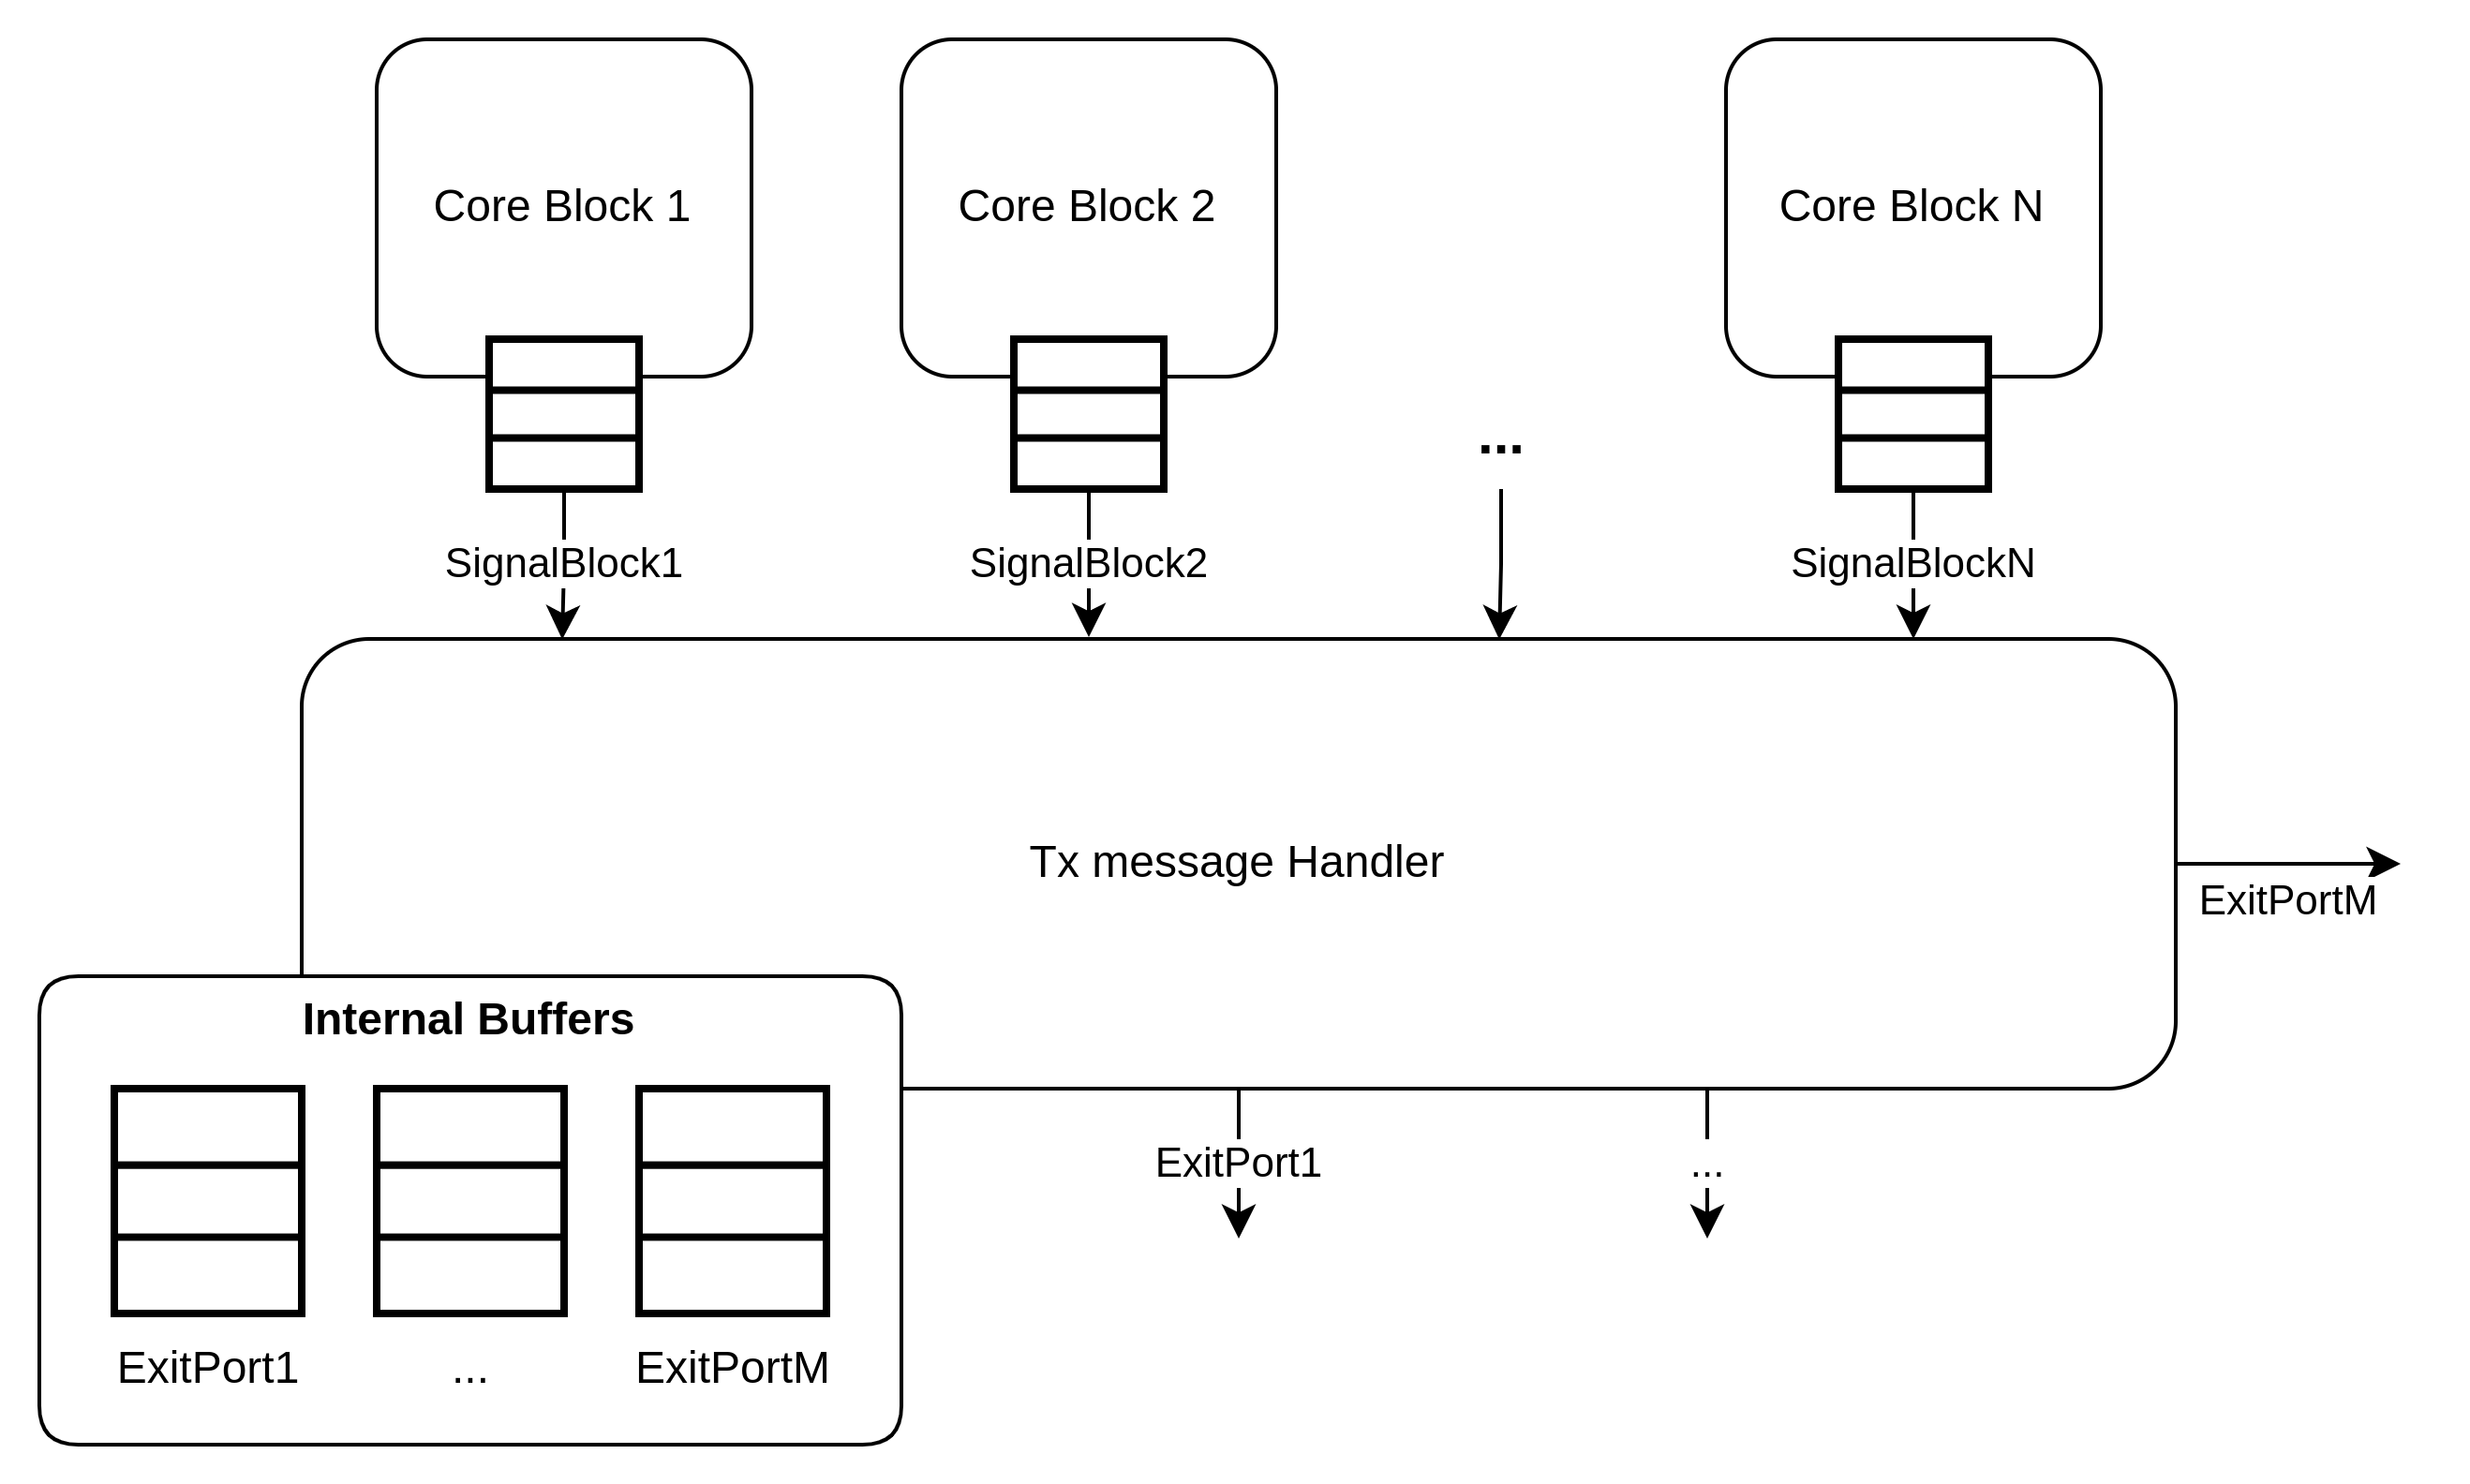
\includegraphics[width=.7\linewidth]{Tx_Message_Handler.png}
	\caption{Message Handler working as Tx}
	\label{fig:tx_message_handler}
\end{figure}

\subsubsection{Rx Mode}
In Rx mode, the Message Handler receives messages from the Tx Message Handler and 
transmits them to the Core Blocks. The diagram of this block can be observed 
in \autoref{fig:rx_message_handler}.
\\
\begin{figure}[H]
	\centering
	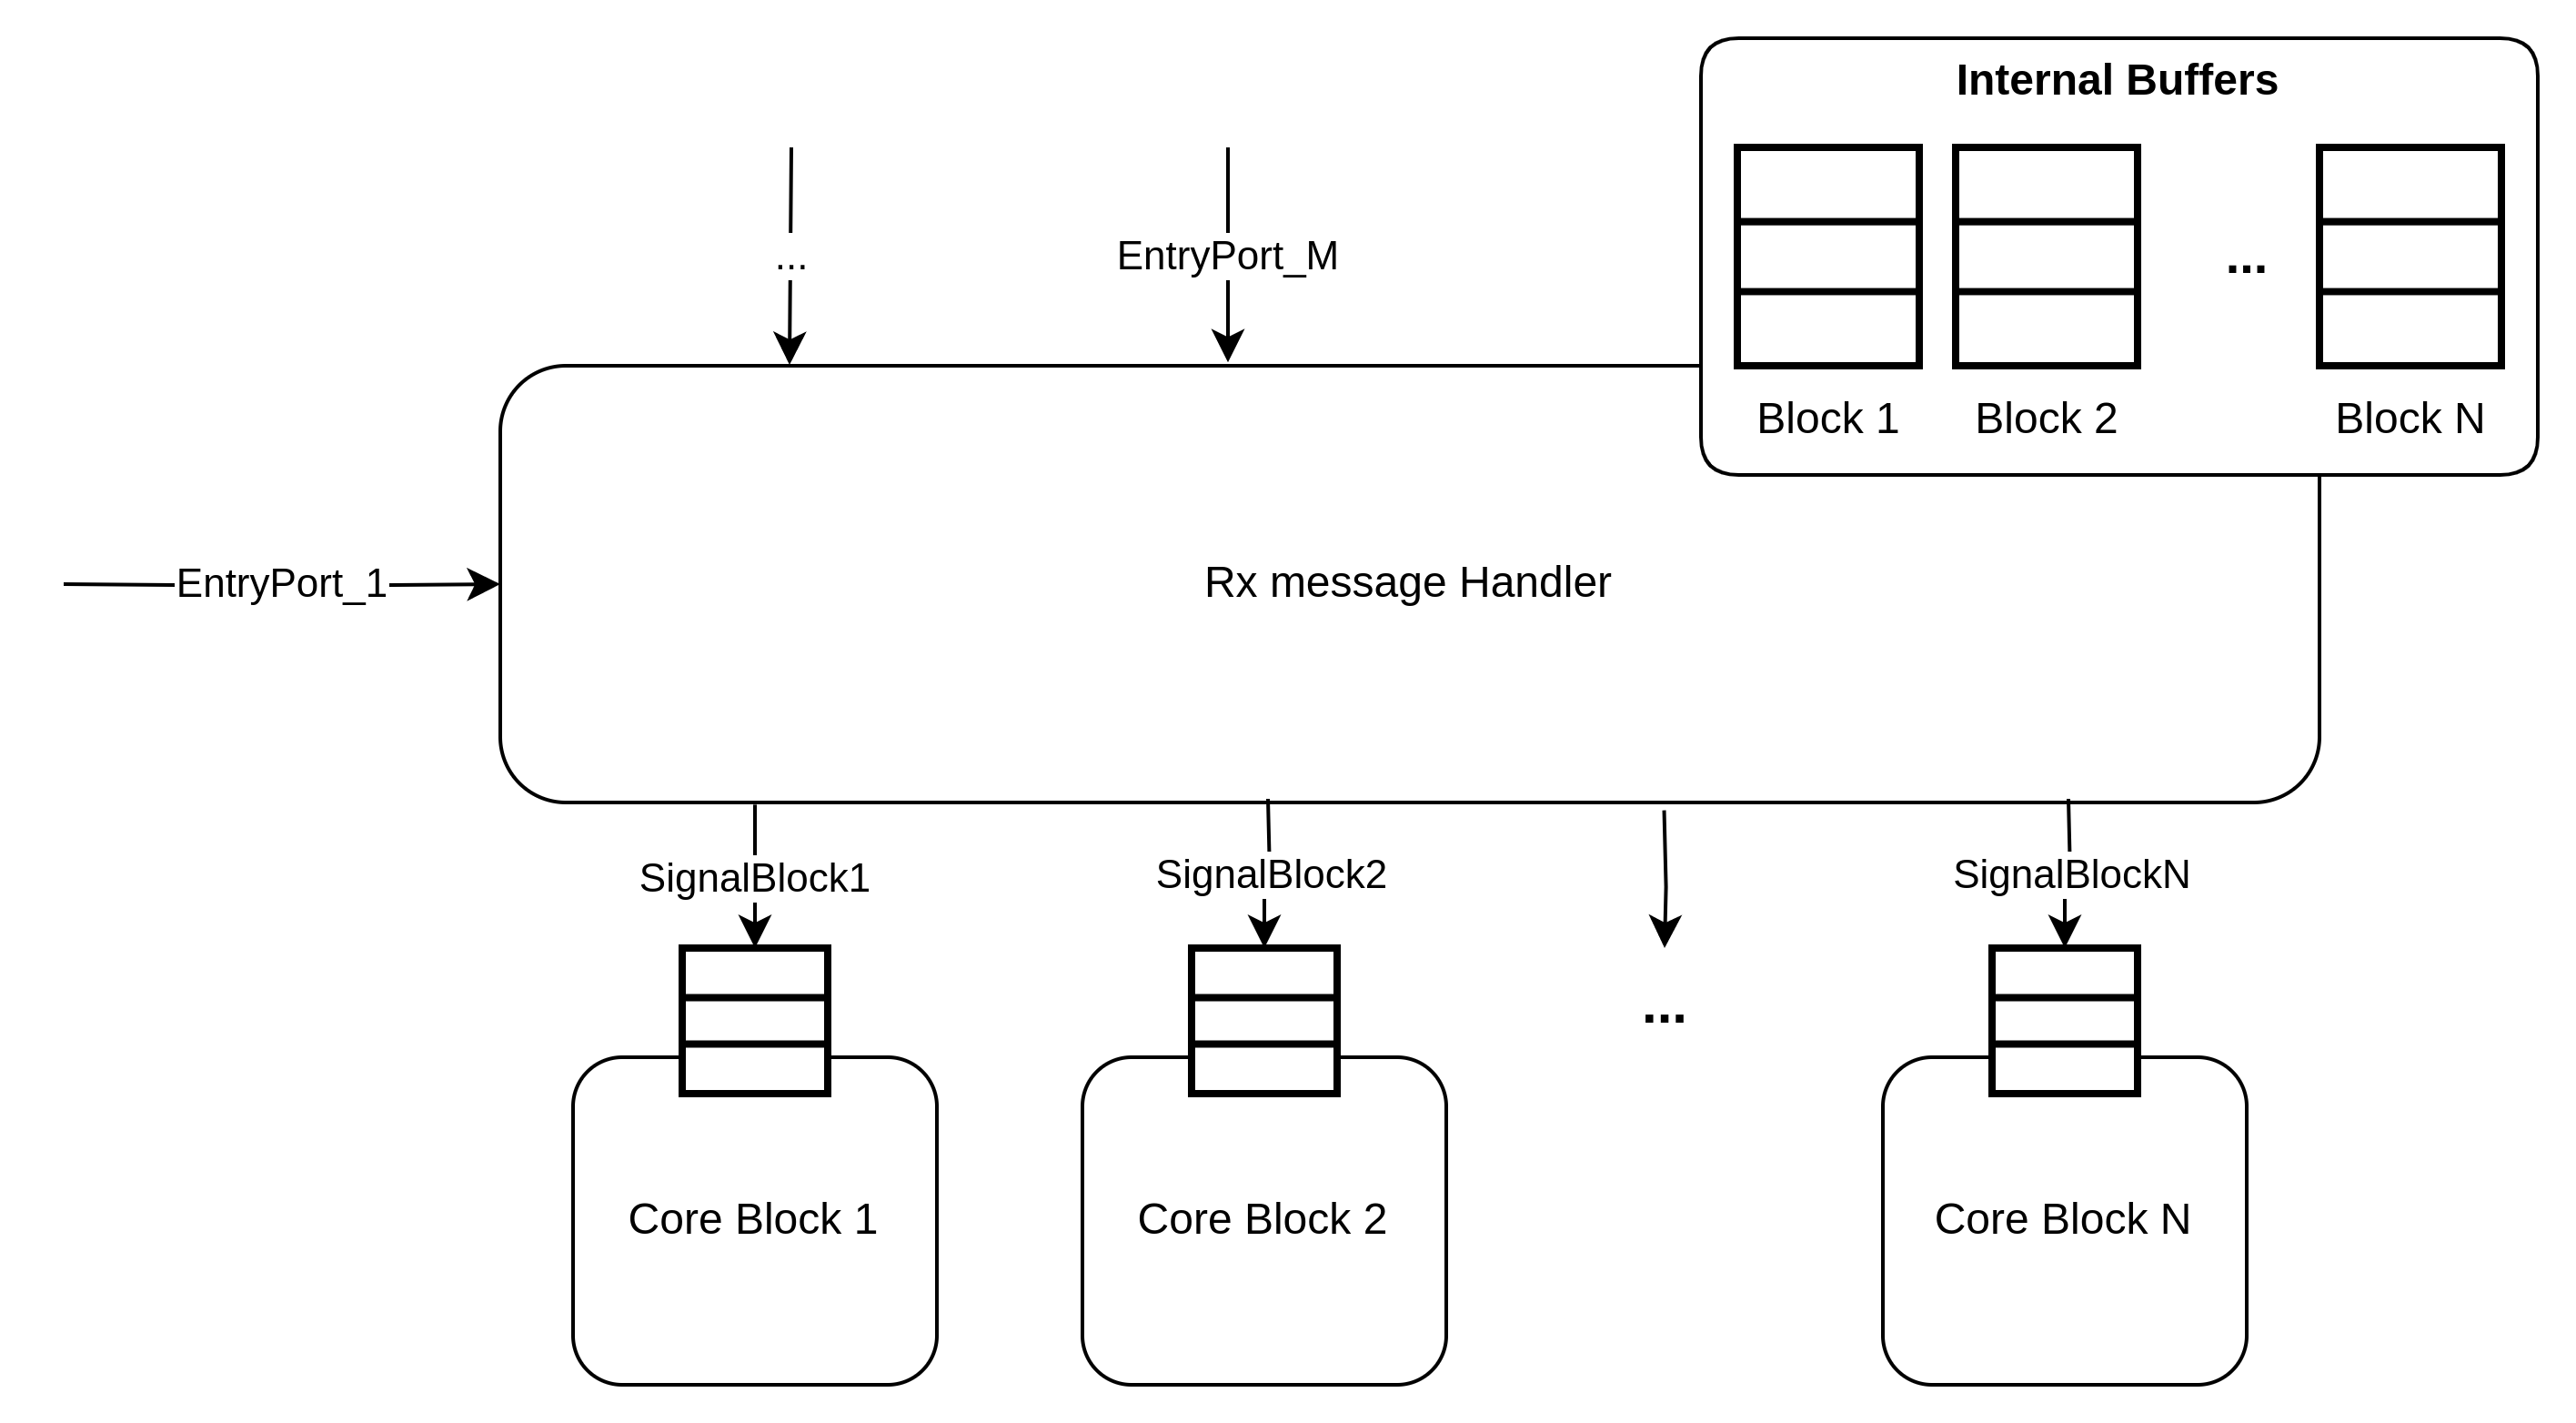
\includegraphics[width=.7\linewidth]{Rx_Message_Handler.png}
	\caption{Message Handler working as Rx}
	\label{fig:rx_message_handler}
\end{figure}

\subsubsection{Automatic Detection of Functioning mode}
When the Message Handler is declared without specifying the functioning mode, it'll 
search for an implicit declaration in the \textit{initialize} function, by analyzing
the types of the Input and Output signals. The options are listed bellow:
\begin{enumerate}
	\item \textbf{Tx} mode, if the Input Signals have different types than \textit{HandlerMessage} 
		and the Output signals are all \textit{HandlerMessage}
	\item \textbf{Rx} mode, if the Input Signals are all of type \textit{HandlerMessage} but the 
		Output signals have different types than \textit{HandlerMessage}
	\item \textbf{Indistinguishable}, if the Input and Output Signals are all of type 
		\textit{HandlerMessage} (Since the types are all equal, there is no need 
		to distinguish between Tx and Rx mode, since the operation is the same)
	\item \textbf{Exception}, if the Input and Output Signals have different types 
		than \textit{HandlerMessage} (A RuntimeError exception is launched and the 
		program is stopped)
\end{enumerate}

%%%%%%%%%%%%%%%%%%%%%%%%%%%%%%%%%%%%%%%%%%%%%%%%%%%%%%%%%%%%%%%%%%%%%%%%%%%%%%
%%%%%%%%%%%%%%%%%%%%%%%%%%%%%% Blocks Execution %%%%%%%%%%%%%%%%%%%%%%%%%%%%%%
%%%%%%%%%%%%%%%%%%%%%%%%%%%%%%%%%%%%%%%%%%%%%%%%%%%%%%%%%%%%%%%%%%%%%%%%%%%%%%

\subsection{Block execution in a project}
The Message Handler and other connected components (Privacy Amplification, 
Parameter Estimation...) are constructed using the block class. This class 
serves as a method to abstractly declare a component and treat it as a separate 
process, however all components still reside in the main process, hence sharing 
the same program memory. Every created blocks needs to have at least two methods, 
\textbf{initialize} and \textbf{runBlock}, for performing actions on the first run
and to execute it subsequently, respectively. This means that in block creation,
we must define clear tasks for the block in each iteration of the \textbf{runBlock} 
function.
\\
The Superblock is just the main block of the project that contain the other blocks
and command their order of execution.
\\
The execution behavior can be observed in \autoref{fig:Blocks_operation_mode}, where
the Superblock will first hand control of execution to the Message Handler and then to
Block 1, Block 2,..., Block N. This execution will be performed until the SuperBlock stops
calling the \textbf{runBlock} method of each block.
\\
\textbf{Note:} The implementation of the components in this project, use the Block 
class, defined in the \textit{Netxpto} file. The order of execution is  
based on the order of declaration of the blocks in the \textbf{MainSystem} class
\\
\begin{figure}[H]
	\centering
	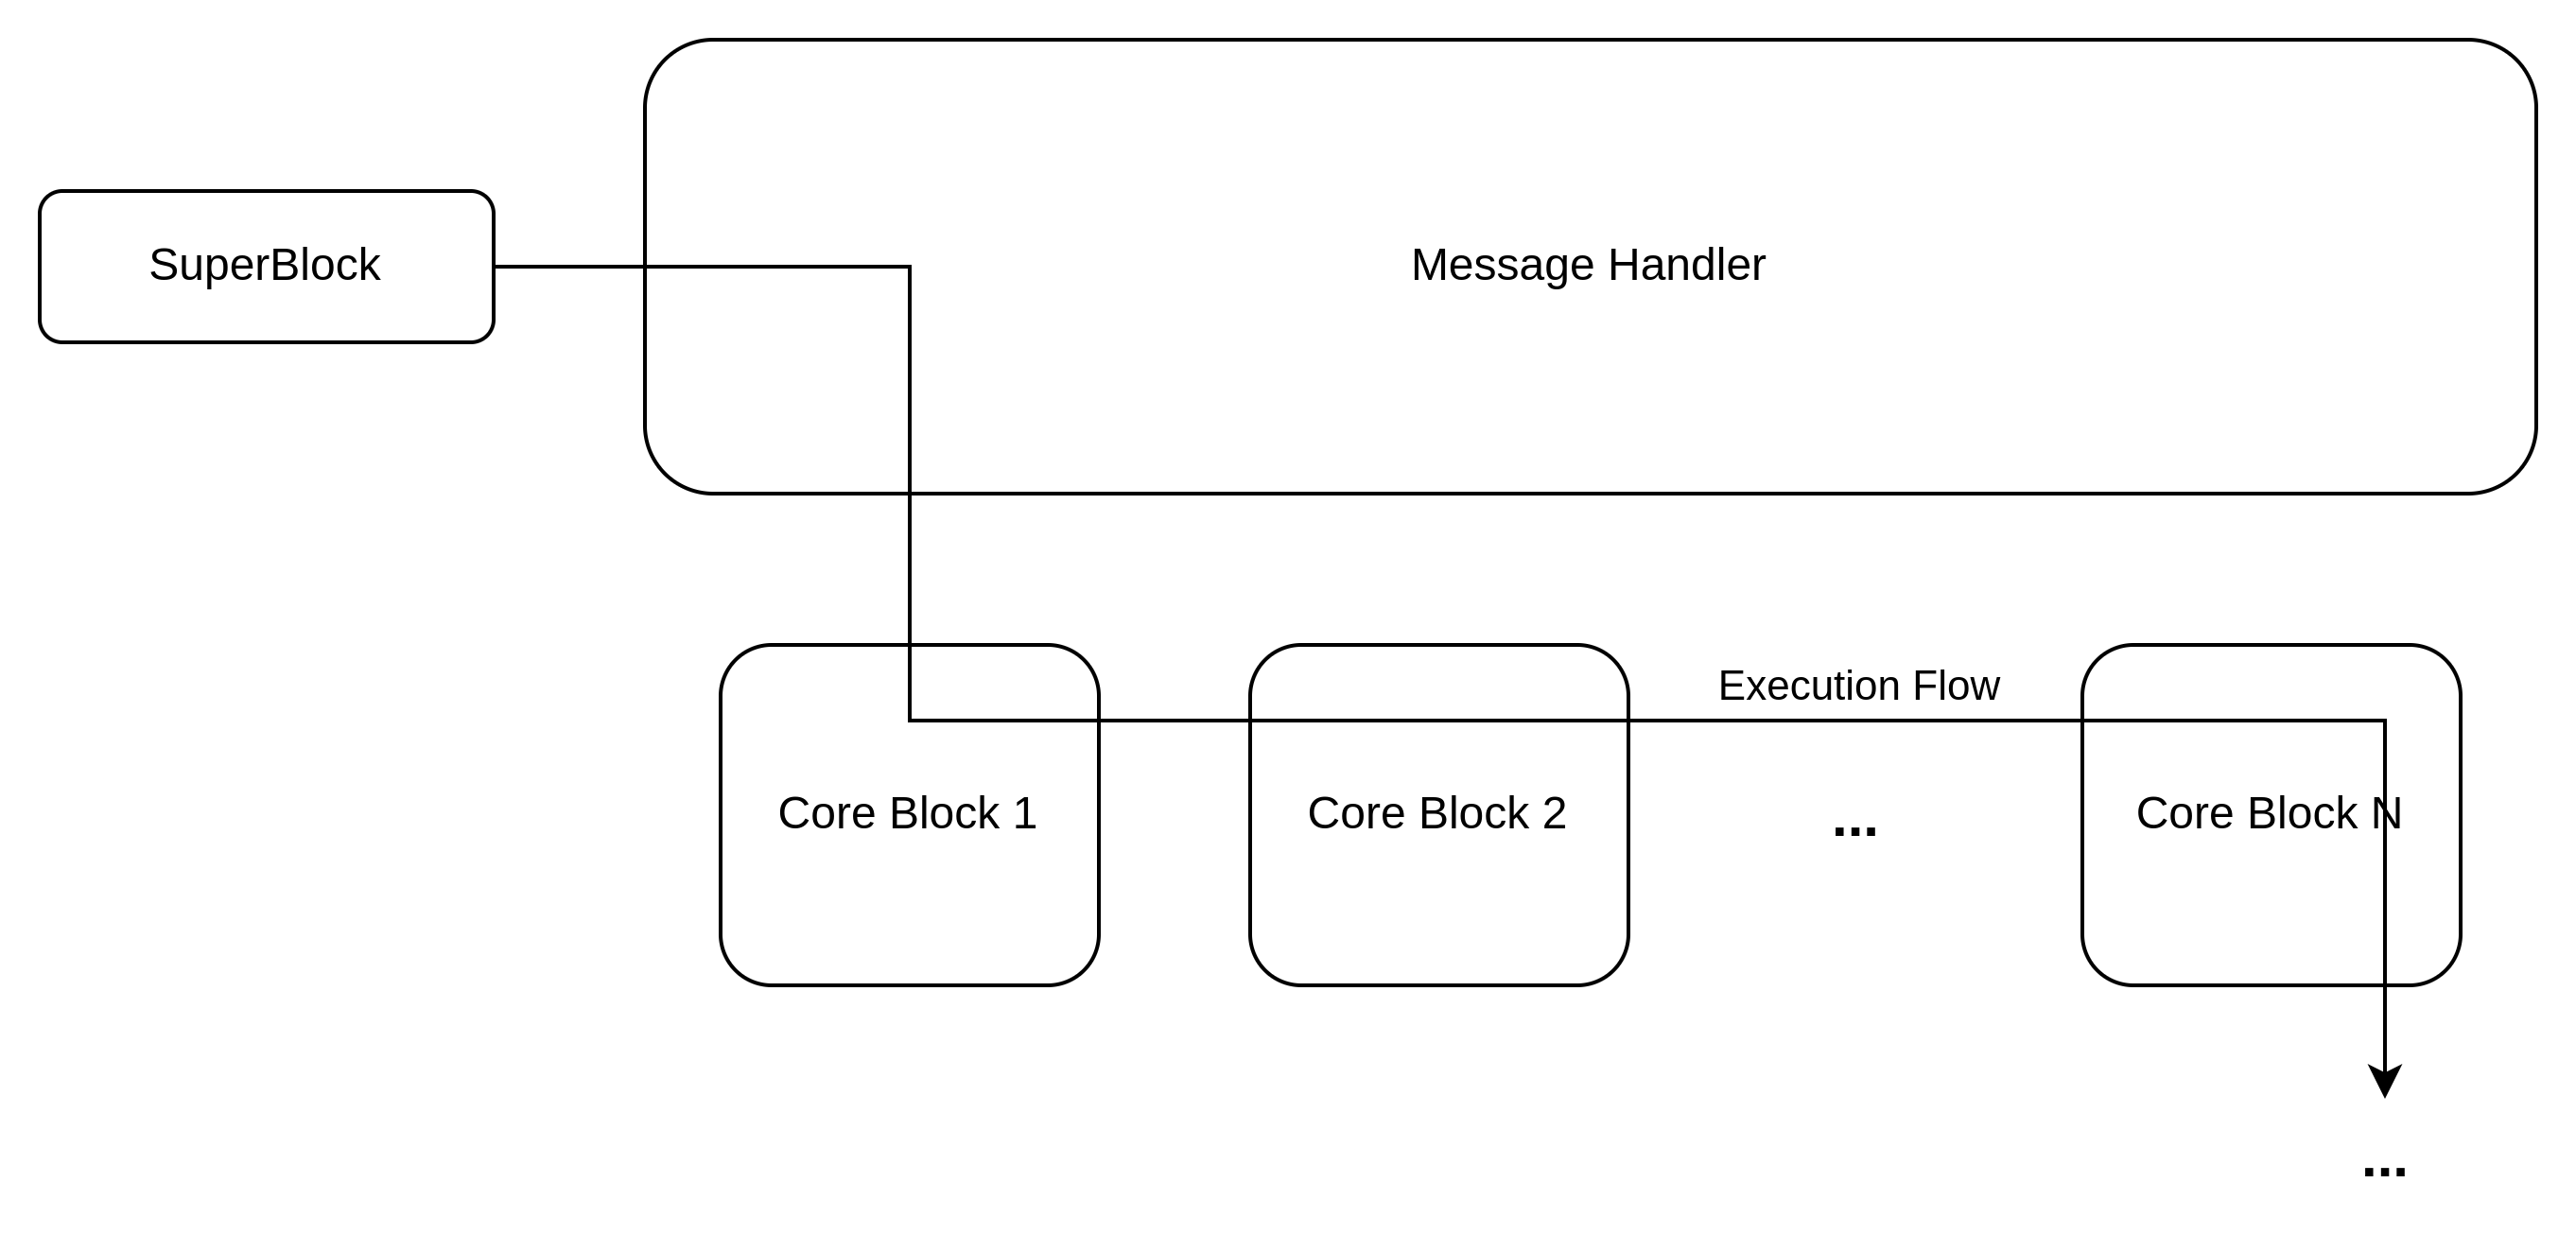
\includegraphics[width=.7\linewidth]{blocks_Operation_Mode.png}
	\caption{Operation mode of the blocks}
	\label{fig:Blocks_operation_mode}
\end{figure}

\subsection{Functional description}
In the initial run, the block will initialize and save the Internal Buffers 
in a list. Take into account that one buffer should be created for each Output 
Signal.
\\
\subsubsection{Running the Block}
The block will start the run by initializing the \textit{Block} \textit{alive} 
attribute to \textbf{false}. The Message Handler will then traverse all 
buffers and try to decrement the priority of all messages with values between 
[1,4]. If any message was decremented, it will then place the \textit{alive} 
value to \textbf{true}.
\\
The next step in execution of the Block is to remove as many messages from the 
internal buffers and place them in the output signals. Then, the Block will 
remove as many messages from the Input Signals, read their destination and 
place them in the internal buffer, according to their destination. Before 
handing execution to the other block, this last step will be repeated.
\\
The flow chart describing the execution is present in 
\autoref{fig:Message_Handler_flow_chart}
\\
\begin{figure}[!b]
	\centering
	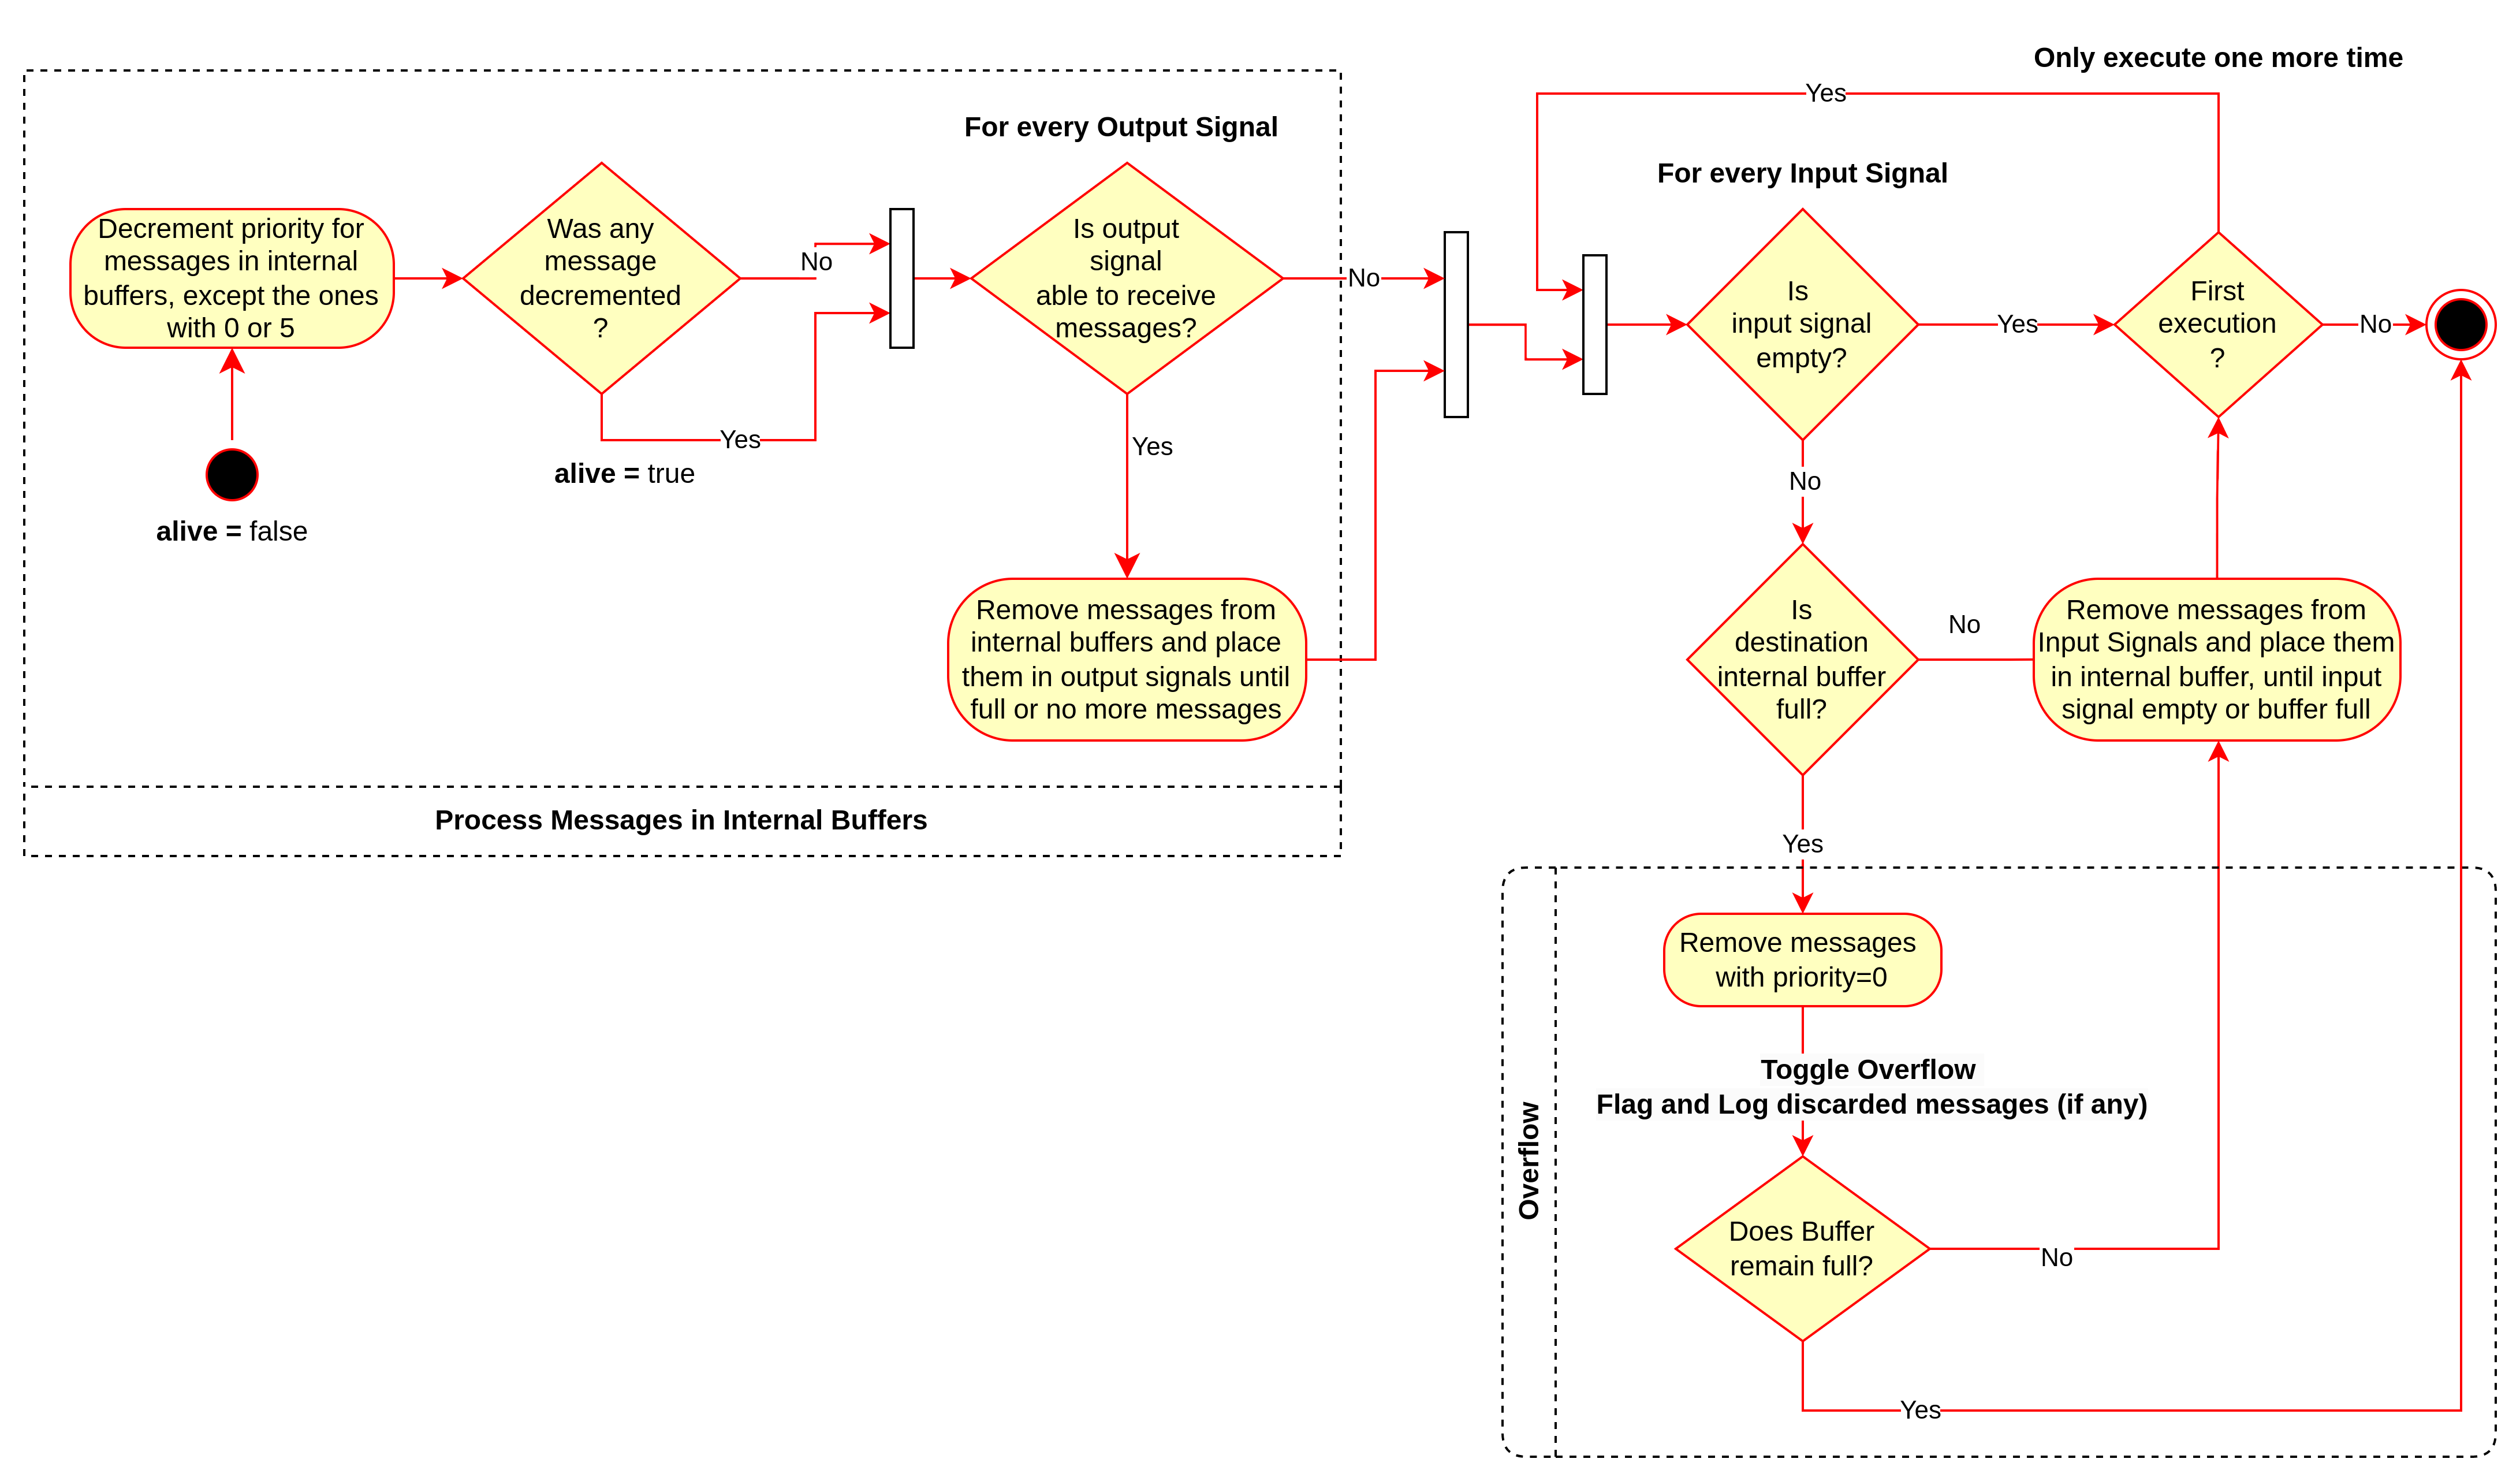
\includegraphics[width=1\linewidth]{flow_chart_message_handler_generic.png}
	\caption{Message Handler functioning flow chart}
	\label{fig:Message_Handler_flow_chart}
\end{figure}
\\
\pagebreak
\\
\subsection{Tests}

Located in this repository, with the path \textit{linkplanner20200819b/doc/tex/lib/message\_handler/tests}, 
there is a project made to test the correct execution of the Message Handler and related
modules.
\\
There were two types of tests developed:
\begin{enumerate}
	\item \textbf{Unit} Tests: found inside the folders \textit{tests}, but not sub-folders
	\item \textbf{End-to-End} Tests: found inside the folder \textit{tests/test\_complete\_system}
\end{enumerate}

\subsubsection{Executing and Compiling}
\label{arc:execComp}
The code developed was created and tested in \textit{Ubuntu 22.04}, using the 
packages \textit{build-essential}, \textit{cmake}, \textit{doxygen}, 
\textit{git} and \textit{Google Tests V1.11.0}.
Most packages can be installed using the following command:
\\
\begin{itemize}
	\item \textit{apt install build-essential cmake doxygen git}
\end{itemize}
\\
For Executing and Compiling the project, take the following steps into account:
\begin{enumerate}
	\item Create a folder named \textit{build}
	\item Navigate to the folder and execute the command \textit{cmake ..}. 
		This step will utilize the CmakeLists to create the compilation 
		environment and create the subsequent auto-generated Cmake files
	\item Next, for compiling the code, run the command 
		\textit{cmake --build .}
	\item After this step, Navigate to the auto-generated \textit{bin/tests} folder
		and chose the executable test to run
\end{enumerate}

\textbf{Note:} There shouldn't be any need to install the \textit{Google Tests V1.11.0} 
package manually, since the CmakeLists is supposed to execute that task.

\subsection{End-to-End tests}

This test is a end-to-end test, meant to represent a full system. This system is represented 
by the \autoref{fig:end-to-end}

\begin{figure}[!b]
	\centering
	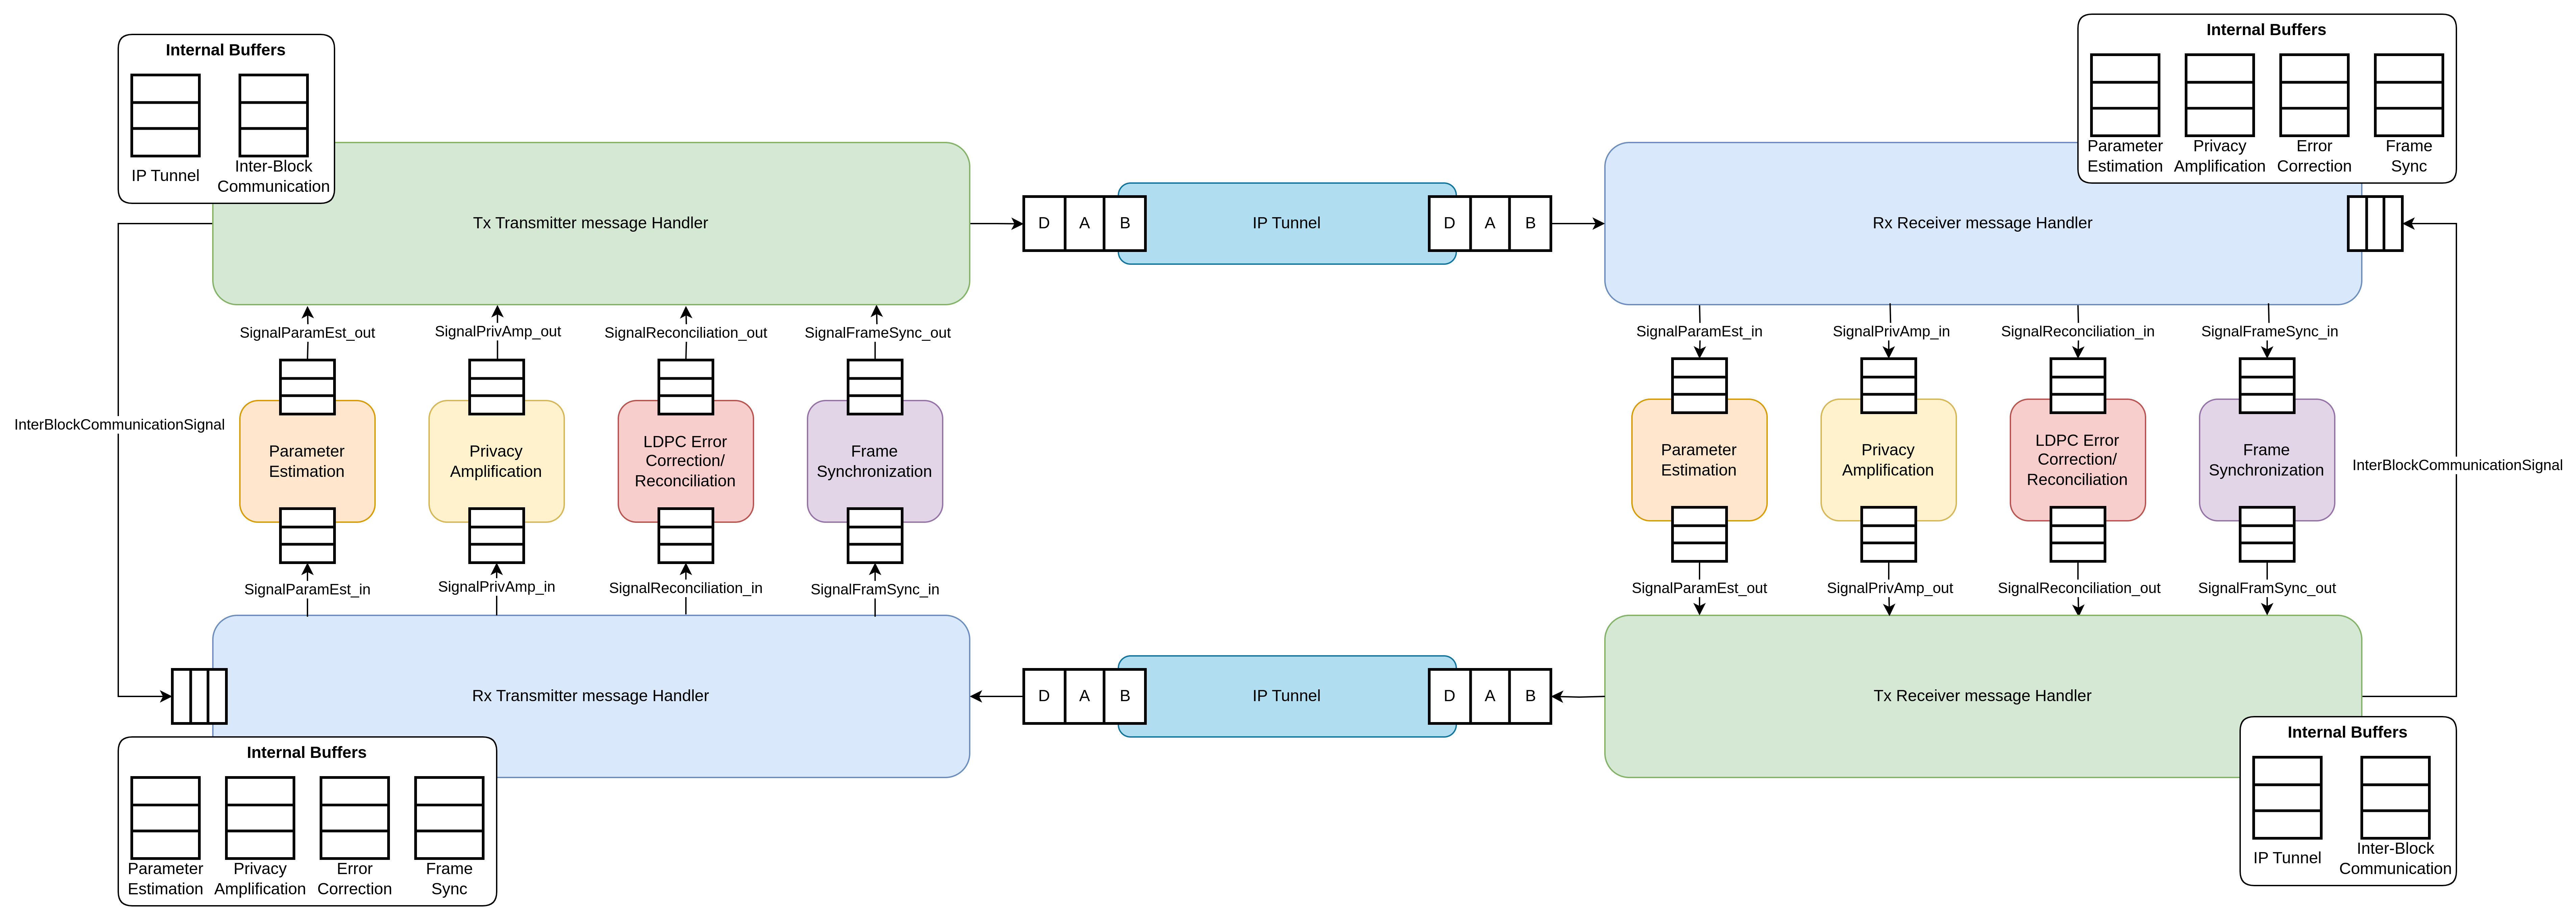
\includegraphics[width=1\linewidth]{end-to-end_test_architecture.png}
	\caption{Full Architecture of the End-to-End test}
	\label{fig:end-to-end}
\end{figure}

\subsubsection{Construction of the System}

The Message Handler was built with modularity in mind, so the tests should also 
take advantage and build upon that basis. 

We started by dividing the system into two main Blocks or \textbf{SuperBlocks} 
and approached two ways on connecting them. In the first, two signals were used, 
allowing almost direct access, bypassing the IP Tunnel. On the second test, the 
IP Tunnel is used, thus allowing to see it's impact on performance. This approach 
rendered a higher level of abstraction, enabling us, in the main test file 
\textit{test\_complete\_system.cpp} to declare, initialize and run the test with 
fewer lines of code and configurations.

\subsubsection{Dummy Block}

The Dummy Block is the representation of a Core Block 
(i.e., Parameter Estimation, Privacy Amplification, etc.). 
This  Dummy Block takes advantage of the class Block defined in the 
\textit{netxpto\_20200819.h} file, mimicking even more a real system. 
\\
A Block is composed of mainly a \textit{initialize}, \textit{runBlock} and 
\textit{terminate} functions that dictate the lifecycle of the Block. Next is 
a brief explanation of each one of this functions:
\\
\begin{enumerate}
	\item \textbf{Initialize}: As the name suggests, it's used to initialize 
		or perform a operation on the first execution of a Block. In this test, 
		no operation is required.
	\item \textbf{runBlock}: The Blocks functions as a Synchronous, single-thread 
		module that offers a degree of abstraction, behaving as if they were a 
		separate process. This means that once they are declared and execution is 
		initiated, they aren't meant to execute for a prolonged time, instead they 
		are supposed to execute and perform some operations and then hand control 
		to the other Blocks. The Dummy Blocks use this function to process messages 
		in the Input Signal and generate messages to be placed in the Output Signals.
	\item \textbf{terminate}: This function is made to signal the termination of 
		the Block. This gives the ability for the Block to perform programmed tasks, 
		such as destroying resources or save it's state. In this case, this function 
		is used to evaluate if there were any lost messages that were sent or messages 
		that were or were waiting to be processed at the time of termination.
\end{enumerate}
\\
In order for the Dummy Block to be generic and represent the various needed Core Blocks, 
when instantiating it, a name can be given. This way, it's a lot easier to assess the 
correct delivery of messages.

\paragraph{Execution in runBlock}

The Dummy Blocks has an internal list, provided by the SuperBlock, that contains 
the possible blocks to send information. It randomly elects a destination Block, 
placing that information in header the data field (Each generated message has an 
ID that is then saved to assert if the message got lost). The receiving block 
will check the destination Block on the header and the data field, assessing if 
he's the intended receiver of the message. If he is, a message will be produced 
and sent as a response. If not, a message will be printed in the screen indicating 
that the message was received by mistake.

\subsubsection{SuperBlock}

The SuperBlock is defined in the \textit{netxpto\_20200819.h} as a Block that is 
composed of a combination of Blocks. Taking advantage of this definition, we 
defined two SuperBlocks:
\begin{enumerate}
	\item \textbf{Left SuperBlock}: Defined in the \textit{left\_superblock.h} file, 
		this Block is composed of all the modules in the left side of the image 
		and handles the execution between them. It also connects to it's Input 
		and Output signals, to be able to communicate with the other SuperBlock. 
		The Blocks managed by this SuperBlock are the following (declared from 
		Top-To-Bottom, like in the \autoref{fig:end-to-end}):
		\begin{enumerate}
			\item Tx Transmitter Message Handler Right - Receives messages from 
				Dummy Blocks and relays them according to the Destination Block
			\item Parameter Estimation Left - Dummy Block that processes and 
				generates messages
			\item Privacy Amplification Left - Dummy Block that processes and 
				generates messages
			\item Error Correction Left - Dummy Block that processes and 
				generates messages
			\item Frame Synchronization Left - Dummy Block that processes and 
				generates messages
			\item Rx Transmitter Message Handler Left - Receives messages from 
				the Output Signals and transmits them to the Dummy Blocks
		\end{enumerate}
\end{enumerate}
\begin{enumerate}
	\item \textbf{Right SuperBlock}: Defined in the \textit{right\_superblock.h} 
		file, this Block is composed of all the modules in the right side of 
		the image and handles the execution between them. It also connects to 
		it's Input and Output signals, to be able to communicate with the other 
		SuperBlock. The Blocks managed by this SuperBlock are the following 
		(declared from Top-To-Bottom, like in the \autoref{fig:end-to-end}):
		\begin{enumerate}
			\item Rx Transmitter Message Handler Right - Receives messages from 
				the Output Signals and transmits them to the Dummy Blocks
			\item Parameter Estimation Right - Dummy Block that processes and 
				generates messages
			\item Privacy Amplification Right - Dummy Block that processes and 
				generates messages
			\item Error Correction Right - Dummy Block that processes and 
				generates messages
			\item Frame Synchronization Right - Dummy Block that processes 
				and generates messages
			\item Tx Transmitter Message Handler Right -  Receives messages 
				from the Dummy Blocks and relays them according to the Destination Block
		\end{enumerate}
\end{enumerate}

\paragraph{Execution in runBlock}

Each execution signalled, the SuperBlock will grant execution time to each 
Block and set the number of messages that each Dummy Block should generate. 

\paragraph{Termination by SuperBlock}

The SuperBlock has two ways to stop the execution:
\begin{enumerate}
	\item Stop the execution abruptly by executing the \textit{terminate} function, 
		checking if any message was lost.
	\item Graceful stop, where the \textit{sendSignalToTerminate} is used to stop 
		the Dummy Blocks from generating new messages but still being able to process 
		and respond to messages. Then the \textit{terminate} function is also used to fully 
		stop the simulation and assess the system state.
		\begin{enumerate}
			\item To ensure a proper termination, the \textit{sendSignalToTerminate} 
				function can be activated to the remaining 5-10\% of iterations, 
				making so that unprocessed messages are less likely to exist.
		\end{enumerate}
\end{enumerate}



\subsection{Further discussion}
If any questions arise from the documentation here present, please head over to 
the source code, where every steps is documented with the intended execution.

\subsection{Future Improvements}
For future Improvements, relating to the Priority Buffer, the insert\_sorted 
function could be optimized, using an insertion algorithm or by checking the 
back of the list and seeing if the message can be placed there with the current 
priority.

\pagebreak

\clearpage

\cleardoublepage
% ---------------------------------------------------------------------

\end{refsection}
% vim: set ts=2 sw=2 tw=80 noet :
